\documentclass[11pt,a4paper]{article}
\usepackage[margin=24mm]{geometry}
\usepackage[T1]{fontenc}
\usepackage[utf8]{inputenc}
\usepackage{lmodern}
\usepackage{microtype}
\usepackage{amsmath,amssymb,amsthm}
\usepackage{booktabs,longtable,tabularx,array}
\usepackage{pdflscape}
\usepackage{graphicx,xcolor,tikz}
\usetikzlibrary{arrows.meta,positioning,calc,fit}
\usepackage{enumitem,fancyhdr,listings}
\usepackage{hyperref}

\definecolor{ink}{HTML}{183247}
\definecolor{teal}{HTML}{168C88}
\definecolor{blue}{HTML}{2B5D89}
\definecolor{light}{HTML}{F1F6F6}
\definecolor{paper}{HTML}{F2F5F8}
\definecolor{muted}{HTML}{657886}
\hypersetup{colorlinks=true,linkcolor=blue,urlcolor=blue,citecolor=blue,
  pdftitle={A common block strategy for hierarchical fast methods},
  pdfsubject={Trees, five design choices, and the mathematics each paper supplies}}
\pagestyle{fancy}
\fancyhf{}
\fancyhead[L]{\small A common block strategy}
\fancyhead[R]{\small Trees and five design choices}
\fancyfoot[C]{\thepage}
\setlength{\headheight}{14pt}
\setlist{nosep,leftmargin=1.6em}
\renewcommand{\arraystretch}{1.16}
\setlength{\emergencystretch}{2em}
\lstset{basicstyle=\ttfamily\footnotesize,breaklines=true,showstringspaces=false,
  frame=single,rulecolor=\color{black!20},backgroundcolor=\color{paper}}
\newcommand{\eps}{\varepsilon}
\newcommand{\nnz}{\operatorname{nnz}}
\newcommand{\T}{\mathsf{T}}
\newcommand{\takeaway}[1]{\begin{center}\colorbox{light}{\parbox{0.96\linewidth}{\vspace{5pt}\centering\textbf{#1}\vspace{5pt}}}\end{center}}

\title{\vspace{-8mm}\LARGE\bfseries A common block strategy\\[3pt]for hierarchical fast methods\bigskip}
\author{\large Trees, five design choices, and the mathematics each paper still has to supply}
\date{\large A readable guide to the framework, the experiments, and Python/Rust implementations}

\begin{document}
\maketitle
\thispagestyle{fancy}
\begin{abstract}
\noindent
Many fast numerical methods face the same difficulty: an interaction matrix has too many entries to form and use directly. A shared strategy is to group rows and columns, compress suitable blocks, and assemble the resulting summaries into an operator or a solver. We organize that strategy into five design choices: \textbf{partition}, \textbf{interaction pattern}, \textbf{representation}, \textbf{sampling}, and \textbf{algebra}. This is a shared language, not a universal solver. Each algorithm gets its power from an additional construction: expansions and translations in FMM; scale-dependent representations in wideband FMM; sparsification and elimination in recursive skeletonization; complementary tilings and nested bases in a butterfly; and residue classes plus Cooley--Tukey recursion in the FFT.

This report explains that shared strategy with explicit calculations, uses butterfly factorization as a worked example of why additional structure is necessary, connects twelve problem-oriented experiments to the five choices, and shows how the same ideas become short Python and Rust implementations with measurable advantages. Small proof sketches and every reported number have corresponding code or audit evidence in this delivery.
\end{abstract}
\vspace{3mm}
\noindent\textbf{Reading route.} Sections 1--3 explain the framework and classical algorithm families. Section 4 derives the butterfly structures. Section 5 presents the experiments by problem. Section 6 describes code and Section 7 summarizes the argument. Appendices A--C contain the Matérn identity, an experiment-by-experiment evidence guide and reproduction commands.
\tableofcontents
\clearpage
\section{The shared problem: too many interactions}

\subsection{What does a block mean?}
Suppose $N$ sources $y_j$ influence $N$ targets $x_i$ through
\begin{equation}
 u_i=\sum_{j=1}^{N}K(x_i,y_j)q_j,\qquad i=1,\ldots,N.
 \label{eq:pairwise}
\end{equation}
In matrix notation, $u=Kq$. A direct implementation stores and applies an $N\times N$ table. \textbf{Applying} the operator means computing $Kq$; \textbf{solving} means finding $q$ such that $Kq=b$. The two tasks share compressed representations, but solving also requires safe elimination and pivoting.

A \emph{block} is a rectangular subset $B=K(X,Y)$ of that table, determined by a row index set $X$ and a column index set $Y$. Its \emph{numerical $\eps$-rank} is
\begin{equation}
 r_\eps(B)=\min\{r:\|B-B_r\|_2\leq \eps\|B\|_2\}.
 \label{eq:numericalrank}
\end{equation}
By the Eckart--Young theorem this is the number of singular values above $\eps\sigma_1(B)$. If $B_r=UV^{\T}$ with $U\in\mathbb R^{m\times r}$ and $V\in\mathbb R^{n\times r}$, one stores $r(m+n)$ rather than $mn$ leading numbers. For complex data, use $UV^*$ where appropriate. \textbf{Exact algebraic rank and numerical $\eps$-rank are different}: the DFT example in Section~\ref{sec:butterfly} makes the distinction visible.

A short representation is therefore not just ``a small rank''. It is a particular stored object, at a stated tolerance and norm, on a stated block geometry. Rank is not an invariant of a PDE alone.

\subsection{A complete example: why some blocks are short}
\label{sec:logexample}
Take $K(x,y)=\log(x-y)$, with $x>0$ and $|y|\le a<x$. Then
\begin{equation}
 \log(x-y)=\log x+\log(1-y/x)
 =\log x-\sum_{q=1}^{\infty}\frac{1}{q}(y/x)^q.
 \label{eq:laplaceseries}
\end{equation}
Every term is a product of a function of $x$ and a function of $y$. Truncating after $q=p$ produces at most $p+1$ separable terms. If $\rho=a/x<1$, the discarded tail obeys
\begin{equation}
 \left|\sum_{q=p+1}^{\infty}\frac{1}{q}(y/x)^q\right|
 \leq \sum_{q=p+1}^{\infty}\frac{\rho^q}{q}
 \leq \frac{\rho^{p+1}}{(p+1)(1-\rho)}.
 \label{eq:logbound}
\end{equation}
That is a complete small compression theorem: \textbf{separation limits $\rho$; a power series gives the representation; the tail bounds the error}. Other kernels need other expansions, bounds and assumptions. Smoothness alone is not a universal compression certificate.

\subsection{Why trees enter}
A single box cannot be far from every target. Hierarchical grouping handles this: small boxes describe local interactions exactly, while larger boxes describe distant ones by short summaries. A parent may reuse information from its children. A tree is therefore an \textbf{accounting device} for covering interactions without treating them all at the most expensive scale; it does not itself prove that a block is low rank.

The rest of the report asks the same five questions of every method.

\section{The five design choices: a common grammar, not a universal recipe}
\label{sec:dials}

\begin{center}
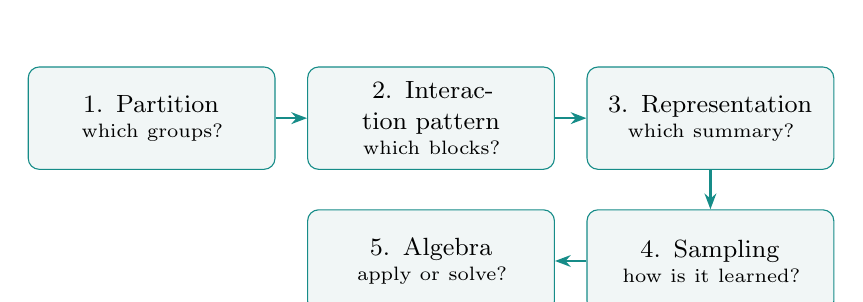
\begin{tikzpicture}[
 font=\small,box/.style={draw=teal,fill=light,rounded corners,align=center,minimum height=13mm},
 every node/.style={align=center}]
\node[box,text width=2.9cm] (p) {1. Partition\\[-2pt]\scriptsize which groups?};
\node[box,text width=2.9cm,right=4mm of p] (a) {2. Interaction pattern\\[-2pt]\scriptsize which blocks?};
\node[box,text width=2.9cm,right=4mm of a] (r) {3. Representation\\[-2pt]\scriptsize which summary?};
\node[box,text width=2.9cm,below=5mm of r] (s) {4. Sampling\\[-2pt]\scriptsize how is it learned?};
\node[box,text width=2.9cm,left=4mm of s] (g) {5. Algebra\\[-2pt]\scriptsize apply or solve?};
\draw[-{Stealth[length=2mm]},thick,teal] (p)--(a);
\draw[-{Stealth[length=2mm]},thick,teal] (a)--(r);
\draw[-{Stealth[length=2mm]},thick,teal] (r)--(s);
\draw[-{Stealth[length=2mm]},thick,teal] (s)--(g);
\end{tikzpicture}
\end{center}

The code calls these choices \textbf{dials}, because several can be swapped while preserving an interface. Mathematically, they are \textbf{design choices}. Each answers a different question; none supplies the evidence needed by the next one.

\subsection{Choice 1: partition and interaction geometry}
\textbf{Question.} Which rows and columns belong together, in which coordinate system and in which order? A spatial binary tree, quadtree or octree groups points by position. A butterfly needs two trees, one for positions and one for frequencies. A transform may instead tree an angle and a spectral degree. The DFT additionally needs bit-reversed index order before residue classes become contiguous intervals.

A partition fixes the candidate blocks, the tree depth, the leaf cost and the opportunities to reuse a parent's work. It does \emph{not} prove that those blocks are compressible. The same matrix with natural, one-sided bit-reversed and two-sided bit-reversed order can have very different numerical $\eps$-ranks (the DFT/FFT ordering experiment). Nor does a smaller leaf or root automatically reduce total work: it also changes the number of blocks and transfers.

\textbf{Failure signal.} Ranks grow because the grouping no longer matches the operator's geometry, or a representation that exists mathematically cannot be reached by the current coordinates. The DFT/FFT experiment responds with residue classes and bit reversal; the spherical-harmonic experiment uses trees in colatitude $\theta$ and degree $l$; the Oseen experiment tests anisotropic geometry near a wake.

\subsection{Choice 2: admissibility and the interaction list}
\textbf{Question.} Which block pairs are compressed, and which are kept explicitly? In one-tree \emph{weak} admissibility, every off-diagonal pair at a parent level is compressed, including touching boxes; leaf and diagonal data remain explicit. In \emph{strong} admissibility, only sufficiently separated pairs are compressed and touching neighbours remain in the near field. The precise distance ratio is an implementation choice. The near/far split determines both approximation work and the exact sparse remainder.

Butterfly \emph{complementary} pairing is different: it is not a Euclidean-distance test. At stage $\ell$ it pairs a row node at depth $\ell$ with a column node at depth $L-\ell$. This produces a sequence of tilings whose row and column widths trade off. Directional rules enlarge or anisotropically deform the near list.

Admissibility does \emph{not} establish the approximation error of an admissible pair, the stability of an elimination, or a cheaper whole algorithm. Strong admissibility, for example, can keep so many near blocks that storage and elimination work rise even when its ranks are smaller (the Oseen wake experiment).

\textbf{Failure signal.} A supposedly admissible block is not low rank, or rank improves but the exact near field dominates. The interaction-geometry experiment changes the rule; the high-frequency-arc experiment uses complementary storage only for separated blocks; the screening experiment allows negligible near blocks to move back into compression.

\subsection{Choice 3: representation and compression}
\textbf{Question.} What mathematical object replaces an admissible block? Three families recur:
\begin{itemize}
 \item \textbf{Analytic summaries.} Multipole/local expansions, plane-wave signatures and their truncation orders. Translation acts on these summaries.
 \item \textbf{Algebraic factors.} $B\approx UV^*$, or an interpolative decomposition (ID) that selects skeleton columns $S$ and represents redundant columns $R$ by $B_{:,R}\approx B_{:,S}T$.
 \item \textbf{Nested representations.} Bases or transfers shared between levels, as in $\mathcal H^2$, HBS and butterfly factorization. Nesting changes the entry count, not merely the rank of an isolated block.
\end{itemize}
The representation determines what is stored and what a transfer means. It does \emph{not} specify how to obtain the factors, how to assemble them, or whether elimination will be stable. An SVD describes an accurate block space; an ID additionally selects rows or columns useful in elimination; neither chooses an FMM translation or a safe pivot.

\textbf{Failure signal.} A single whole-block low-rank factor needs rank growing with frequency (the high-frequency-arc experiment), independent tiles need too many separate bases (butterfly), or block-valued and multi-order kernels do not fit a scalar single-order representation (Stokes and Matérn sampling).

\subsection{Choice 4: sampling and construction}
\textbf{Question.} Which data determine the representation, and what entries or operator products must be read? Exact sampling reads true far-block rows. Proxy sampling evaluates auxiliary points on a circle, sphere, annulus, lifted surface or volume. Randomized construction uses matrix--vector products or sketches. Entry-sampled butterfly constructors use selected entries and require their own coherence hypotheses.

Sampling is both a \textbf{mathematical sufficiency hypothesis} and a \textbf{cost model}. A proxy is sufficient only if observations on the auxiliary set determine the fields that matter at the true far points. A cheap factor is not cheap to build if its constructor still reads all $N^2$ entries. Conversely, an exact far-block ID can be accurate yet interact badly with a later complex elimination (complex Helmholtz elimination).

Sampling does \emph{not} follow from kernel smoothness, does not certify a solve, and does not inherit an arbitrary block's relative scale safely. In exponentially small blocks, a per-tile relative tolerance can waste rank or generate non-finite factors (screened kernels and spherical harmonics). A robust rule needs an absolute or global reference scale as well as floating-point safeguards.

\textbf{Failure signal.} More proxy points on the same set do not improve the answer (fractional/Riesz interactions), a two-sided kernel loses its row relations (Lippmann--Schwinger scattering), tiny matrices become subnormal (screened kernels and spherical harmonics), or a cheap representation costs too much to construct (the spherical-harmonic experiment's all-order precomputation).

\subsection{Choice 5: algebra and assembly}
\textbf{Question.} How do the local representations become an apply, transform or solve? Assembly is not interchangeable bookkeeping. It determines the data flow and the extra stability questions:
\begin{itemize}
 \item FMM translates and accumulates expansions without eliminating sources.
 \item Butterfly and FFT multiply a chain of sparse factors.
 \item Recursive skeletonization and FMM-LU sparsify, eliminate redundant unknowns, track Schur fill and finish with triangular/root solves.
\end{itemize}
Algebra does \emph{not} inherit stability from an accurate apply. Solving amplifies errors through conditioning and pivots. It also changes cost accounting: a smaller Schur root can coexist with larger storage and elimination work.

\textbf{Failure signal.} Pivots deteriorate even though $\|A_{\rm fast}-A\|$ is small (complex Helmholtz elimination), an approximate inverse fails at a caustic (the high-frequency-arc experiment), or a quantity of interest is accurate while the underlying density is not (the Oseen wake experiment).

\subsection{The algebra choice contains three assembly grammars}
\label{sec:grammars}
It is useful to make the three data flows explicit. They share block vocabulary but are not one universal algorithm.

\paragraph{G1: sum over levels (FMM and $\mathcal H^2$).}
Schematically,
\begin{equation}
 A\approx A_{\rm near}+\sum_{\ell=1}^{L}R_\ell^{\T}
 \left(\bigoplus_{\tau}T_{\ell,\tau}\right)S_\ell,
 \label{eq:g1}
\end{equation}
where $S_\ell$ forms source summaries, $T_{\ell,\tau}$ translates them across the interaction list, and $R_\ell$ distributes local information to targets. Upward merging, translation and downward inheritance are the algorithm.

\paragraph{G2: product of sparse factors (butterfly and FFT).}
The matrix becomes a chain such as
\begin{equation}
 A\approx U_LG_{L-1}\cdots G_hM_hH_h^*\cdots H_{L-1}^*V_L^*.
 \label{eq:g2}
\end{equation}
Application means applying the chain. Complementary low rank makes its local blocks small; nesting and radix recursion determine why the whole chain is cheap.

\paragraph{G3: eliminate (HBS, recursive skeletonization and FMM-LU).}
After row/column sparsification, redundant variables are eliminated. The basic Schur step is
\begin{equation}
 \begin{bmatrix}P&Q\\R&S\end{bmatrix}
 \begin{bmatrix}a\\b\end{bmatrix}=\begin{bmatrix}f\\g\end{bmatrix}
 \quad\Longrightarrow\quad
 (S-RP^{-1}Q)b=g-RP^{-1}f.
 \label{eq:schur}
\end{equation}
Repeating it bottom-up produces a direct factorization. Pivots, fill-in and modified blocks are now part of the representation, not an implementation afterthought.

\subsection{Three independent certificates}
A useful performance report maintains three separate budgets:
\begin{enumerate}
 \item \textbf{Approximation:} achieved error against a trusted reference at a stated tolerance and norm;
 \item \textbf{Stability:} safe pivots, conditioning and meaningful output errors for a solve;
 \item \textbf{Total cost:} construction, storage, application or solve work, and memory.
\end{enumerate}
A low rank is useful evidence for the first budget; it does not, by itself, certify the other two. A single accounting form is
\begin{equation}
 C\approx C_{\rm near}+C_{\rm build}
 +\sum_{\ell}n_\ell c_\ell C_{\rm transfer}(r_\ell)+C_{\rm root},
 \label{eq:costaccounting}
\end{equation}
where $n_\ell$ is the number of boxes at level $\ell$, $c_\ell$ the number of compressed partners per box, and $r_\ell$ their summary size. Every method needs this product, not just its $r_\ell$.

\section{From the same grammar to different algorithms}
\label{sec:algorithms}

\subsection{FMM: a tree of useful expansions}
The fast multipole method starts with a spatial tree, exact near interactions and separated far interactions. The expansion of a source box gives its outgoing summary; a translation sends it to another box; a local expansion evaluates its influence on target points. Its operation names have intuitive meanings:
\begin{itemize}
 \item sources to multipole (S2M): build a leaf's outgoing summary;
 \item multipole to multipole (M2M): re-express a child at its parent;
 \item multipole to local (M2L): translate an outgoing expansion into a local one;
 \item local to local (L2L): send inherited local information to children;
 \item local to target (L2T): evaluate potential where it is needed.
\end{itemize}
This is G1 from \eqref{eq:g1}. The logarithmic example above is a toy one-dimensional version of the same principle. The essential paper-specific contribution is \textbf{analytic representation and translation theory}: choices of centers, orders, transforms, error bounds and reuse. One tree and one admissibility rule do not derive those operators.

For a standard full-grid FMM same-level candidate list, the bound is $6^d-3^d$: 27 in two dimensions and 189 in three. With fixed expansion order in a non-oscillatory regime, the number of boxes decreases geometrically up the tree and the work can total $O(N)$. That is a statement about both the list and the transfer cost, not a consequence of the tree alone.

\subsection{Wideband FMM: change translation and representation with scale}
\label{sec:wideband}
Oscillatory kernels need more detail than the logarithmic example. Write a 3-D surface problem's top-level width in wavelengths as $W=kD/(2\pi)$ up to the report's convention; the essential scaling is $W\propto kD$. A large-box partial-wave order has leading form
\begin{equation}
 p=O\big(W+\log(1/\eps)\big),\qquad (p+1)^2\ \text{coefficients}.
\end{equation}
This leading large-box statement does not say that the separate low-frequency exponential expansions are accuracy-independent.

At high frequency, an ordinary expansion may be expensive to translate. A plane-wave or far-field-signature representation makes each direction-scale interaction almost \textbf{diagonal}: multiply each sampled direction independently. For a surface discretization with $N\propto(kD)^2$, the contrast is schematically
\begin{equation}
 \sum_\ell4^\ell(kw_\ell)^3=O(N^{3/2})
 \quad\text{versus}\quad
 \sum_\ell4^\ell(kw_\ell)^2=O(N\log N),
 \label{eq:wideband-cost}
\end{equation}
over the high-frequency levels; bounded-order finer levels add $O(N)$. Thus changing translation can matter more than changing rank.

At small scales, diagonal plane-wave forms can lose accuracy through cancellation and overflow before truncation. The wideband construction therefore combines low-frequency exponential/partial-wave machinery with high-frequency directional forms, conversion rules and filtering. The cited implementation's transition scales are $0.25$, $3.50$ and $12.0$ wavelengths at requested accuracies $10^{-3}$, $10^{-6}$ and $10^{-9}$, respectively \cite{cheng2006wideband}. They are measured transition choices, not one universal $\lambda/4$ rule. Its stated complexity is $O(N)$ when low-frequency work dominates and $O(N\log N)$ when high-frequency work dominates.

In our language:
\[
\text{FMM assembly}+\text{scale-appropriate expansions}
+\text{diagonal translations}+\text{a stable switch}.
\]
The major gain lies in representation and translation, not only in rank.

\subsection{Recursive skeletonization: use redundancy to eliminate}
\label{sec:rskel}
For unknowns $B$ inside a box, an ID chooses skeleton columns $S$ and redundant columns $R$ so that, against a far set $F$,
\begin{equation}
 A_{F,R}\approx A_{F,S}T.
 \label{eq:idrelation}
\end{equation}
Thus $S$ is a small set of interactions representing the rest against $F$. Nonsymmetric matrices need row as well as column control: the teaching driver stacks the two interaction directions rather than assuming symmetry.

Sparsification makes redundant unknowns couple only weakly to $F$. Block Gaussian elimination \eqref{eq:schur} then removes them, propagates skeletons upward and ends with a dense root solve. This is G3, not ``FMM run backwards'' in any literal sense \cite{ho2012hife,minden2017rss}. The new requirements are:
\begin{itemize}
 \item an elimination order that controls fill-in;
 \item stable pivots and conditioning estimates, not only small interpolation error;
 \item a list of blocks already changed by earlier Schur updates;
 \item singular and near-singular quadrature, which changes the original near entries.
\end{itemize}
In strong-admissibility FMM-LU, the modified-block or $Q$ set must include the appropriate non-kernel entries from the \emph{current} working matrix \cite{sushnikova2023fmmlu}. A proxy built only from the original kernel cannot see those Schur-generated entries unless the driver supplies them.

\clearpage
\begin{landscape}
\begin{table}[p]
\centering\footnotesize
\setlength{\tabcolsep}{3pt}
\caption{The complete algorithm map. ``G1/G2/G3'' refers to Section~\ref{sec:grammars}. The last column is the essential content that a generic block/tree interface does not supply.}
\label{tab:algorithm-map}
\begin{tabular}{@{}>{\raggedright\arraybackslash}p{1.55cm}>{\raggedright\arraybackslash}p{2.75cm}>{\raggedright\arraybackslash}p{2.65cm}>{\raggedright\arraybackslash}p{3.55cm}>{\raggedright\arraybackslash}p{3.45cm}>{\raggedright\arraybackslash}p{2.55cm}>{\raggedright\arraybackslash}p{5.85cm}@{}}
\toprule
Method & Partition / geometry & Interaction rule & Representation / compression & Sampling / construction & Assembly / grammar & Extra mathematics contributed by the algorithm \\
\midrule
FMM & One spatial tree shared by sources and targets & Exact near list; separated same-level far list & Outgoing/multipole and incoming/local analytic expansions & Kernel expansion formulas and quadrature; orders chosen by truncation bounds & \textbf{G1}: S2M, M2M, M2L, L2L, L2T & Addition/translation theorems, stable recurrences, expansion-order error bounds, interaction-list scaling and reuse. \\
Wideband FMM & FMM spatial tree with low- and high-frequency levels & Same near/far lists, but representation and regime switch depend on box size in wavelengths and $\eps$ & Low-frequency exponential/partial-wave forms; high-frequency plane-wave/far-field signatures; diagonal translators & Direction samples, interpolation/filtering and conversion between representation families & \textbf{G1} with scale-specific M2L and conversions & Stable diagonal translation, conversion/interpolation on the sphere, cancellation analysis and the precision-dependent switch. \\
HBS, RS, FMM-LU & One tree; nested skeletons per box & Weak off-diagonal or strong separated pairs; level-restricted strong lists; modified near blocks & ID skeletons $S,R$, interpolation $T$, Schur complements and LU factors & Exact true rows, proxy rows/volumes, sketches; current-$Q$ entries must be supplied in strong elimination & \textbf{G3}: sparsify, eliminate, triangle solves and dense root & Elimination order, fill-in/$Q$ bookkeeping, stable pivots, proxy representation theory and singular/near quadrature. \\
Butterfly & Two trees: row depth $\ell$ paired with column depth $L-\ell$ & Complementary phase-space tilings, not a distance predicate & Local low-rank tiles plus nested bases and small cross-level transfers & Full tile entries in our teacher; random products or sampled entries under separate hypotheses in fast constructors & \textbf{G2}: a product of $O(\log N)$ sparse factors & Phase regularity/complementary low rank, middle-level split, basis recursion, merge formulas and construction cost/incoherence theory. \\
FFT & Two index trees in mutually matched bit-reversed order & Complementary residue classes at every stage & Exact rank-one character tiles and diagonal twiddles & Exact index arithmetic; no statistical sampling & \textbf{G2}: Cooley--Tukey even/odd half-transforms and recombination & The residue identity \emph{and} radix recursion $T(N)=2T(N/2)+O(N)$, twiddle algebra and output permutation. \\
\bottomrule
\end{tabular}
\end{table}
\end{landscape}

\paragraph{Implementation boundary.} Table~\ref{tab:algorithm-map} is an algorithmic reading map, not a feature list for the included code. The Python package contains representative tree/admissibility/ID/proxy, recursive-solve and interpolative-butterfly drivers; it does not contain production FMM or wideband translation machinery. Rust contains smaller real-kernel examples, direct FFT/DFT-butterfly examples and a separate feasibility core. Section~\ref{sec:implementations} states exactly which library routine each shipped example reuses.

\takeaway{A shared data structure and measurement framework makes the algorithms easier to compare; it does not remove the expansions, translations, nested transfers, elimination theory or index recursion that make them work.}

\section{Butterfly as a worked derivation: why extra structure is necessary}
\label{sec:butterfly}

The butterfly is especially instructive because its first calculation can look like generic low-rank compression, while its speed comes from a second piece of organization. Start with
\begin{equation}
 K(x,\xi)=e^{2\pi i\Phi(x,\xi)},\qquad f=Kg.
 \label{eq:fiokernel}
\end{equation}
Rows correspond to positions $x$, columns to frequencies $\xi$. We follow Li, Yang, Martin, Ho and Ying's \emph{Butterfly Factorization} \cite{li2015butterfly}, while placing each construction step into the shared grammar.

\subsection{Two trees and the mixed phase}
There is no reason to use the same hierarchy for both variables: positions and frequencies have different roles. Let a tile have centers $(x_0,\xi_0)$ and define its nonseparable remainder by
\[
R(x,\xi)=\Phi(x,\xi)-\Phi(x,\xi_0)-\Phi(x_0,\xi)+\Phi(x_0,\xi_0).
\]
Then exactly
\begin{equation}
 e^{2\pi i\Phi(x,\xi)}
 =e^{2\pi i\Phi(x,\xi_0)}e^{2\pi iR(x,\xi)}
 e^{2\pi i(\Phi(x_0,\xi)-\Phi(x_0,\xi_0))}.
 \label{eq:phasepeel}
\end{equation}
The two one-variable factors are diagonal row and column scalings: they cannot change singular values or rank. Only the mixed remainder controls how many local patterns are required. If $\left|\partial_x\partial_\xi\Phi\right|\leq M$ and tile widths are $w_A,w_B$, the mixed-difference bound is
\begin{equation}
 |R(x,\xi)|\leq \frac{M}{4}w_Aw_B.
 \label{eq:phasebound}
\end{equation}
For the bilinear phase $\Phi=x\xi$, $R=(x-x_0)(\xi-\xi_0)$, so $\exp(2\pi iR)$ has a converging separated exponential series. Hence a small tile area gives a short sum in a completely explicit calculation.

For a general phase, this motivates what to measure; it does not replace the rank theorem's additional smoothness/analyticity hypotheses \cite{candes2009butterfly}. ``One phase-space cell has rank one'' is intuition; the peeled mixed phase is the rigorous object.

\subsection{Complementary tilings: thinner rows require wider columns}
The complementary rule pairs a row node at depth $\ell$ with a column node at depth $L-\ell$ of two binary trees, where $L=\log_2N$. Tile areas proportional to $N$ then keep the phase variation in \eqref{eq:phasebound} controlled. Narrower position boxes are paired with wider frequency boxes. Unlike weak/strong rules, this is not a Euclidean distance condition.

Figure~\ref{fig:two-trees} makes the index geometry explicit at $N=8$, so $L=3$. Moving down the position tree splits a row interval; the partner sits higher in the frequency tree, so the column interval merges. At the selected stage $\ell=2$, $A$ is a depth-two position interval with $|A|=2$, while $B$ is a depth-one frequency interval with $|B|=4$. Across $\ell=0,1,2,3$, the shapes are $8\times1$, $4\times2$, $2\times4$ and $1\times8$: every tile has eight entries, but a different aspect ratio. It is this \textbf{entry area} $|A||B|$ that the normalized phase/peeling argument controls.

The second tree is therefore not decorative. It supplies exactly the complementary blocks on which low rank is tested. The nested transfers below then explain why moving through these pairs is useful \emph{globally}: local bases are connected across stages instead of being rebuilt independently.

\begin{figure}[htbp]
\centering
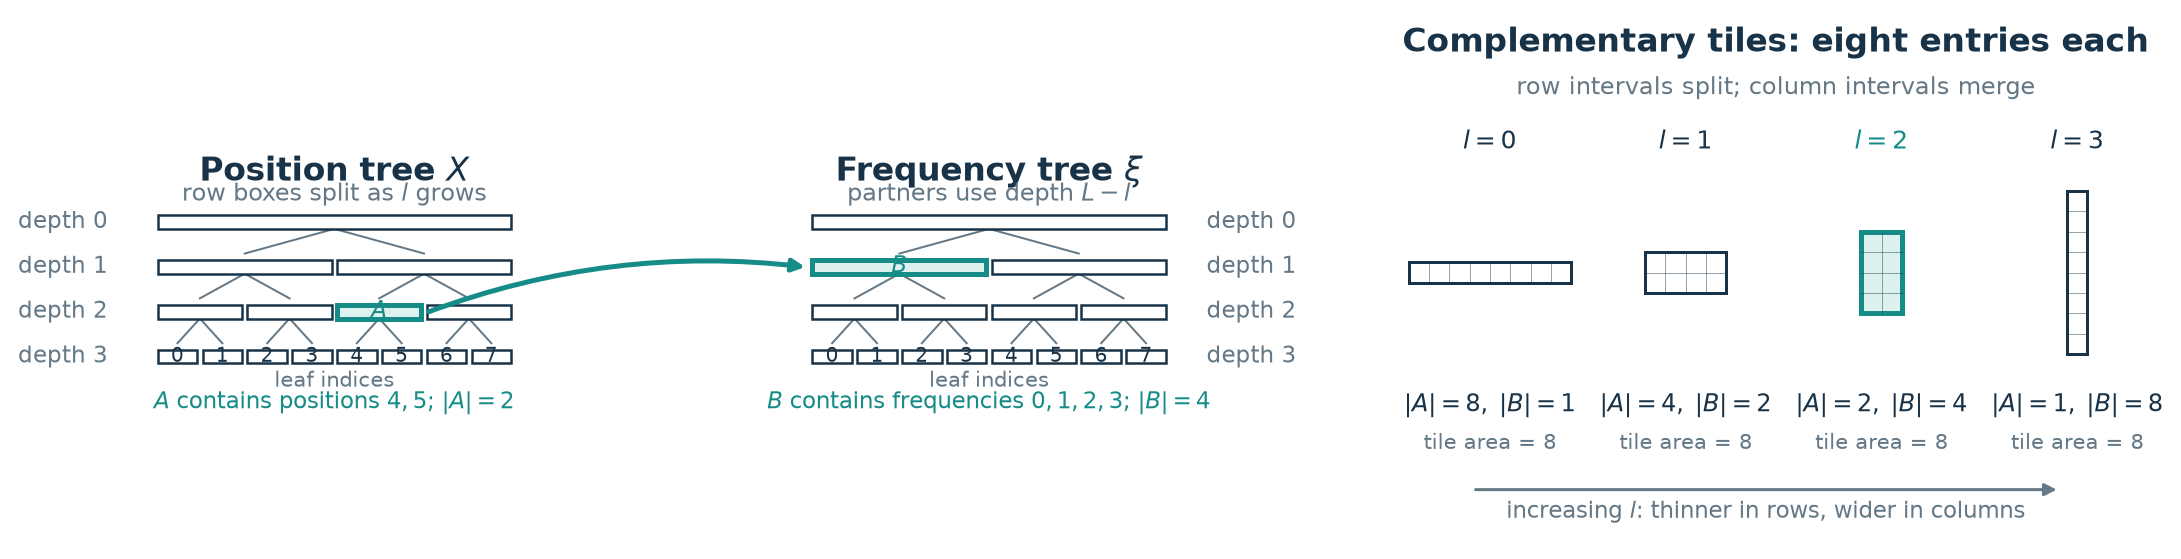
\includegraphics[width=\linewidth]{figures/two-trees.png}
\caption{The two binary trees and their complementary tilings. The selected pair has depths $\ell=2$ and $L-\ell=1$ for $L=3$. Row intervals split with depth; their column partners merge. Each displayed tile has eight entries, while its aspect ratio changes. The figure describes index geometry, not a general rank theorem.}
\label{fig:two-trees}
\end{figure}

Figure~\ref{fig:tiling} compares a fixed tiling with the middle complementary tiling at tolerance $10^{-6}$. The same kernel and same direct rank measurement lead to very different conclusions.

\begin{figure}[htbp]
\centering
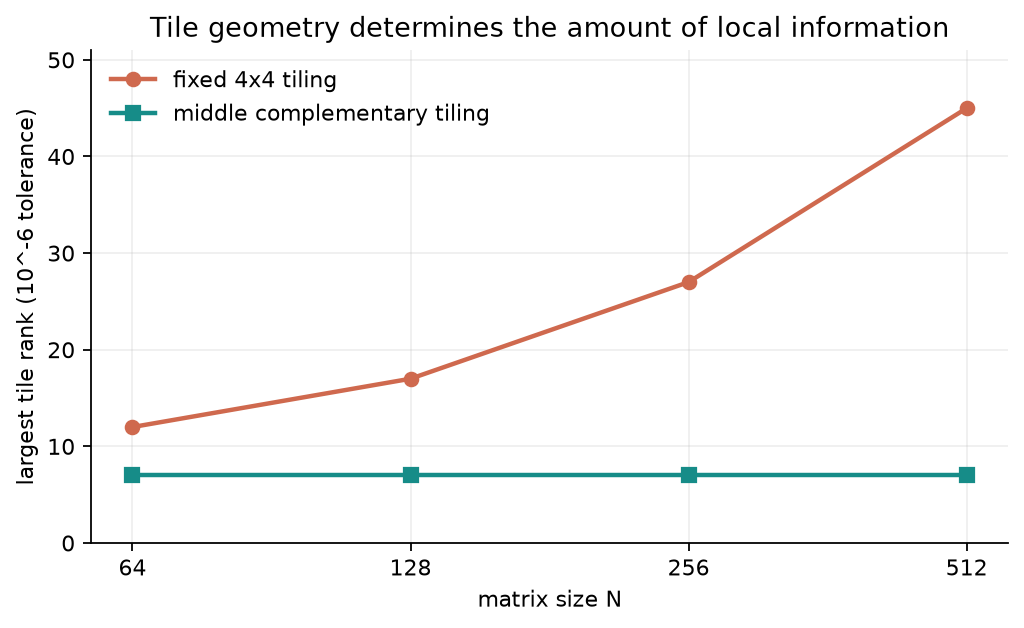
\includegraphics[width=0.87\linewidth]{figures/tile-ranks.png}
\caption{A bad tiling cannot always be repaired by a better compressor. Here the maximum rank grows with $N$ in a fixed $4\times4$ tiling but is nearly constant in a middle complementary tiling. Data: \texttt{results/butterfly-discovery-ranks.json}.}
\label{fig:tiling}
\end{figure}

\subsection{Representation first: local low rank is not yet a fast algorithm}
At the middle level, if $L$ is even, there are $N$ square tiles of size $\sqrt N\times\sqrt N$. One rank-$r$ tile has $O(r\sqrt N)$ leading factor entries; this is not an assertion that constructing it from the full tile costs only that much. Across all tiles, independent storage and apply work total
\begin{equation}
 N\times O(r\sqrt N)=O(rN^{3/2}).
 \label{eq:middlecost}
\end{equation}
This is \textbf{useful}: middle-level splits and low ranks are real. It is not yet $O(N\log N)$, because there are too many independent bases and local products. The paper responds by recursively factorizing the left and right bases, rather than doing more independent SVDs.

\subsection{Nesting gives speed}
Suppose two old summaries $c_1,c_2$ feed a new tile. Their contributions can be re-expressed in the new tile's small basis $U_{\rm new}$:
\begin{equation}
 U_1c_1+U_2c_2\approx U_{\rm new}(T_1c_1+T_2c_2).
 \label{eq:transfer}
\end{equation}
The small transfer matrices $T_1,T_2$ reuse earlier work instead of constructing a new summary from scratch. Repeating this relation through both trees yields nested bases and a ladder of sparse factors.

If old ranks are $r_0,r_1$ and the new rank is $r_2$, one merge has at most
\begin{equation}
 r_2(r_0+r_1)
 \label{eq:transfercost}
\end{equation}
stored entries before zero and identity entries are removed. With bounded ranks, $O(N)$ entries per stage and $O(\log N)$ stages give $O(N\log N)$ storage and apply work. This is the precise meaning of:
\takeaway{Tiles give low rank; nesting gives speed.}

Our small Python driver uses a one-sided column-ID version of this nesting. The reference paper's middle-out construction is more symmetric and contains the precise recursions. These two descriptions share structure but are not identical algorithms.

\subsection{Sampling and construction remain a separate budget}
Three access models deserve different cost estimates:
\begin{itemize}
 \item \textbf{All entries read.} Simple, deterministic and general. Reading a dense matrix already costs $\Theta(N^2)$. Our teaching/reference builder uses all rows of every tile; it is not the reference paper's optimal construction.
 \item \textbf{Black-box products.} Random probes against $K$ and $K^*$ identify local spaces. For an $N\times N$ matrix with bounded tile ranks, the paper's matrix-product construction has $O(N^{3/2}\log N)$ work when its required fast operator products have unit accounted cost \cite{li2015butterfly}.
 \item \textbf{Sampled entries.} Its sampled-entry route obtains $O(N^{3/2})$ construction under its coherence hypotheses. Row-sampled interpolative methods provide another route with a different access model \cite{pang2018idbf}.
\end{itemize}
The common grammar deliberately separates \textbf{representation} (what is stored) from \textbf{sampling} (how it is obtained). A fast apply does not automatically pay back an expensive construction.

\subsection{The FFT supplies an exact special case}
Let $N=2^L$ and $F_{jk}=e^{2\pi ijk/N}$. Choose residue classes
\[
j=a+2^\ell u,\qquad k=b+2^{L-\ell}v.
\]
Then
\[
\frac{jk}{N}
=\frac{ab}{N}+\frac{av}{2^\ell}+\frac{bu}{2^{L-\ell}}+uv.
\]
Because $uv\in\mathbb Z$, $\exp(2\pi iuv)=1$. Every complementary tile is \textbf{exactly} rank one: a tile constant, a row-only vector and a column-only vector. Bit reversal makes these residue classes contiguous. Reversing only one tree is insufficient.

This exact statement must not be confused with a numerical rank in another ordering. A contiguous natural-order tile is exactly full rank on its short side by a Vandermonde argument, although its short-arc Fourier nodes are ill conditioned: at $N=256$, its numerical $10^{-12}$-ranks across the stages are $1,2,4,8,11,8,4,2,1$. If one block is a residue class and the other is contiguous, the mixed matrix is a full Fourier block: at the middle of $N=1024$ both its exact and numerical ranks are $32$. Thus both-tree bit reversal creates an identity; one-sided reversal does not merely lose a constant factor.

For rank-one tiles, factors store $N$ at $W$, $2N$ at each of $L$ intermediate $G_\ell$, and $N$ at $U$. Therefore
\begin{equation}
 \nnz=2N\log_2N+2N.
 \label{eq:fftcount}
\end{equation}
Cooley--Tukey even/odd recombination supplies the actual FFT algorithm \cite{cooley1965fft}. With $E$ and $O$ the length-$N/2$ transforms of the even and odd inputs and $\omega_N=e^{2\pi i/N}$, the sign convention above gives
\begin{equation}
 (F_Ng)_j=E_j+\omega_N^jO_j,\qquad
 (F_Ng)_{j+N/2}=E_j-\omega_N^jO_j,
 \qquad 0\le j<N/2.
 \label{eq:cooley-tukey}
\end{equation}
Reusing the two half-transforms gives $T(N)=2T(N/2)+O(N)=O(N\log N)$. The residue identity supplies exact rank-one tiles; \eqref{eq:cooley-tukey} supplies the recursive algorithm. The count \eqref{eq:fftcount} describes the factor representation; an in-place FFT does not need to materialize the full factor chain.

\begin{figure}[htbp]
\centering
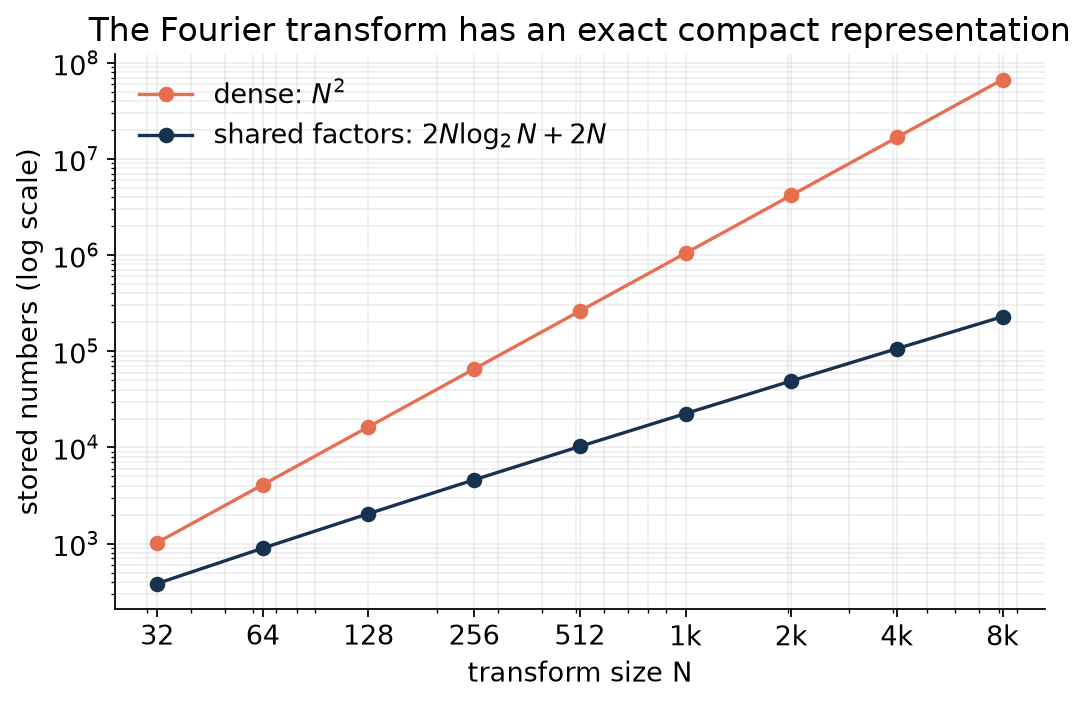
\includegraphics[width=0.82\linewidth]{figures/dft-storage.png}
\caption{Exact DFT factor storage compared with dense. Both Python and Rust independently check rank one at every stage and reconstruction of the underlying DFT operator.}
\label{fig:dftstorage}
\end{figure}

\section{Experiments by problem: where generic choices fall short}
\label{sec:experiments}

The experiments are not twelve demonstrations that one preset solver works everywhere. They are twelve diagnostic cases: begin with a shared block strategy, identify the assumption that fails, and isolate the additional object that repairs or explains it. The object may be an identity, a different geometry, a representation, a tolerance rule or a cost distinction.

For every experiment below, the same four questions are answered: \textbf{What is the interaction? What generic choice is made first? Where is it insufficient? What new mathematics enters, and which measured result can actually be cited?} ``Measured'' always refers to the stated finite problem, tolerance and implementation. ``Proved'' refers only to the displayed identity or argument. Neither label is a claim of literature-first novelty.

\subsection{The essential diagnostic map}
\begin{longtable}{@{}>{\raggedright\arraybackslash}p{0.20\textwidth}>{\raggedright\arraybackslash}p{0.26\textwidth}>{\raggedright\arraybackslash}p{0.32\textwidth}>{\raggedright\arraybackslash}p{0.13\textwidth}@{}}
\toprule
Observed shortfall & The generic assumption that failed & Additional mathematics or design response & Problem \\
\midrule
\endhead
Rank or storage grows with $N$ & One off-diagonal geometry fits every kernel and ordering & Match phase-space tiles and index order to the operator; distinguish exact from numerical rank & Geometry, DFT order, arcs \\
Local tile ranks are bounded but there are too many independent bases & Low-rank tiles alone imply a fast global apply & Two complementary trees, recursive basis nesting and small transfer matrices & Spherical harmonics \\
A proxy does not determine the true far field & Auxiliary evaluations of a smooth kernel are automatically sufficient & Exterior representation/uniqueness, a two-sided kernel, richer sample volume, or related kernel orders & Proxies, Riesz, scattering, Matérn \\
Tiny blocks inflate in rank or produce non-finite factors & A tolerance relative to each tile's largest pivot is safe and efficient & Absolute/global scaling and a floating-point floor & Screening, harmonics, Matérn \\
An accurate apply gives an unstable elimination & Representation accuracy implies pivot stability & Adjoint congruence, real interpolation and separate pivot/condition checks & Complex Helmholtz \\
Anisotropy should reduce every cost & A smaller root or fewer skeletons means a cheaper solve & Directional near boxes and proxy curves, plus separate near-field, storage, root and elimination budgets & Oseen; screening \\
A good functional implies a good solution everywhere & One error metric certifies the whole computation & Name the quantity of interest; separately measure density, conditioning and physical discretization & Stokes, Riesz, scattering, Oseen \\
A fast factorization repays its construction & Stored factors and apply cost determine total performance & State the access model and construction cost separately, including recurrence tables and dense work arrays & FFT alternatives, arcs, harmonics \\
\bottomrule
\end{longtable}

This table is the main sense in which the framework is constructive: it says \textbf{where to look next}. It does not choose the next theorem automatically.

\subsection{Experiment: Which interaction geometry fits which kernel?}
\label{exp:e1}
\paragraph{Interaction and generic start.} The study forms the same matrix three ways for Laplace, Helmholtz, Gaussian and Fourier-integral kernels. Trees and the per-block numerical-rank rule are fixed at $\eps=10^{-6}$. Weak admissibility compresses off-diagonal box pairs; strong admissibility compresses only separated pairs; complementary pairing uses row depth $\ell$ with column depth $L-\ell$. Storage is counted per point over $N=256,\ldots,4096$.

\paragraph{Where the generic choice falls short.} It is tempting to declare that strong admissibility is right for smooth kernels and complementary admissibility is right for oscillatory kernels. The data reject that as a universal rule. A Helmholtz boundary kernel has singular diagonal tiles for which complementary pairing is inappropriate, while nesting makes a storage comparison depend on format as well as geometry.

\paragraph{Additional mathematics.} The needed idea is \textbf{phase-space interaction geometry}, not a stronger compressor. Complementary tiles control the mixed phase of Fourier-type far interactions; strong admissibility protects near-singular boundary interactions. This comparison also requires an accounting distinction: weak/strong numbers here use flat, non-nested factors, whereas the complementary numbers are entries in a nested butterfly chain.

\paragraph{Checked result and boundary.} At $N=4096$, DFT storage per point is $2886$ weak, $1543$ strong and $629$ complementary, with maximum numerical ranks $1045$, $275$ and $18$: the stored-number ratios are $4.59$ and $2.45$. For the Helmholtz curve at ten points per wavelength, strong stores $566$ per point and complementary $666$, with the same fitted storage exponent $1.40$; diagonal complementary tiles reach full numerical rank $141$. The supported conclusion is ``match the interaction pattern to the kernel and region'', not ``complementary always wins'' and not a ranking of flat H-storage against nested HBS/$\mathcal H^2$.

\subsection{Experiment: DFT ordering, radix recursion, and FFT alternatives}
\label{exp:e2}
\paragraph{Interaction and generic start.} The operator is
\[
 K(x,\xi)=\exp\{2\pi i(x\xi+t\,c(x)|\xi|)\},\qquad \eps=10^{-6}.
\]
At $t=0$ it is the DFT. The first generic choice is a butterfly in natural order. The second is an alternative representation: approximate the non-DFT phase by $\sum_{r=1}^R a_r(x)b_r(\xi)$ and apply $R$ FFTs with diagonal scalings.

\paragraph{Where the generic choice falls short.} A generic complementary low-rank statement does not choose the index ordering. Natural-order DFT tiles have numerical $\eps$-rank about eight in this driver; reversing just one tree gives a full Fourier block. The FFT representation also does not tell us when $R$ separate FFTs are cheaper than one butterfly.

\paragraph{Additional mathematics.} Two exact structures enter. First, residue classes make DFT tiles exactly rank one, as derived in Section~\ref{sec:butterfly}; matched bit reversal makes those classes contiguous, and Cooley--Tukey recursion supplies the algorithm. Second, the $R$-FFT route is governed by the perturbation's phase range $B=t\,\Delta c\,N/2$, not simply by how rough $c(x)$ looks. The measured fit is $R\approx B+O(\log(1/\eps))$ over the tested media.

\paragraph{Checked result and boundary.} In matched bit-reversed order, every DFT tile has exact rank one and stored entries are exactly
\[
 2N\log_2N+2N=4608,\quad22528,\quad106496
 \qquad(N=256,1024,4096),
\]
with measured apply errors $2.6\times10^{-14}$ to $4.1\times10^{-13}$. Natural order needs $11.3$--$18.5$ times as many entries in the same ID-butterfly driver. For the sine medium at $N=4096,t=1$, $B=256$, $R=275$ and the $R$-FFT apply costs $16$ times the butterfly's accounted complex multiply-adds. Apply break-even occurs around $R\approx10$--$17$, or $B\lesssim2$--$8$ in this sweep. Storage break-even is much later ($B\approx245$--$294$ for the sine at $N\ge2048$), and construction is not included. Bit reversal is not universal: at $t>0$ the tested bit-reversed FIO tiles become full rank.

\subsection{Experiment: Deciding whether a proxy determines the far field}
\label{exp:e3}
\paragraph{Interaction and generic start.} Recursive skeletonization is held fixed at $N=2048$, $\eps=10^{-8}$, maximum leaf size 32. Three compressors are compared: exact IDs of true far rows; 64-point proxy circles at radius $2.5$ box half-widths, with required explicit rows; and Gaussian-sketch IDs. The test matrices include Laplace, outgoing Helmholtz, nonsymmetric double-layer/advection--diffusion, Gaussian RBF and Cauchy-type kernels.

\paragraph{Where the generic choice falls short.} ``The kernel is smooth away from the diagonal'' does not imply that a proxy circle determines the far field. Under strong admissibility the proxy carries essentially the entire far interaction, so any missing exterior representation becomes visible. A second, narrower failure occurs on real wave kernels when a radial factor vanishes on the proxy radius.

\paragraph{Additional mathematics.} The proxy hypothesis is an \textbf{exterior representation theorem}: for a Green's kernel, a source field outside a box can be represented by appropriate data on an auxiliary boundary. It is not a symmetry condition. Where no such representation determines the field, exact or randomized sampling supplies the missing span. For real $Y_0$/$J_0$ kernels, two rings change the radial zeros and repair the single-ring resonance. Stability of the subsequent complex elimination is a different question and is isolated in the complex-elimination experiment.

\paragraph{Checked result and boundary.} On the non-PDE Gaussian/Cauchy sweep, single-circle proxy solve errors are $1.7\times10^{-7}$ to $4.3\times10^{-5}$, or $17$--$4300$ times $\eps$; exact and randomized variants stay at most $5\times10^{-10}$ on these inputs. On the tested exterior-PDE kernels the proxy meets tolerance and uses $3$--$13$ times fewer modeled compression flops than exact sampling. At $Y_0(kR)=0$ the measured proxy error is $6\times10^{-4}$; two rings reduce the cited $Y_0$ case to $2\times10^{-13}$, with $3\times10^{-10}$ for $J_0$. The failure band in relative detuning is measured to be at most about $1.5\times10^{-7}$. Exact sampling here is an oracle for comparison, not a claim of a cheap production constructor.

\subsection{Experiment: Butterfly-compressed far blocks and approximate inverses}
\label{exp:e4}
\paragraph{Interaction and generic start.} This experiment has two linked problems. First, a separated 2-D Helmholtz block $(i/4)H_0^{(1)}(k|x-y|)$ on two arcs is stored either as one whole-block ID or as a butterfly in the two arc parameters, at ten points per wavelength and achieved error at most $10^{-6}$. Second, the 1-D FIO from the DFT/FFT ordering experiment is solved by GMRES using butterfly applies at tolerance $10^{-8}$.

\paragraph{Where the generic choice falls short.} The whole block's numerical rank grows with frequency, so its storage eventually loses to complementary tiles. But low rank alone does not supply that crossover, and a good apply does not supply a good inverse. At a caustic the ray map folds and the forward operator itself becomes ill conditioned.

\paragraph{Additional mathematics.} For storage, the new objects are \textbf{complementary phase-space tiles and nested bases}; equal achieved errors and identical identity-entry accounting are required for a fair ratio. For the solve, the adjoint $K^*/N$ exploits near-unitarity away from caustics. The ray-Jacobian-weighted adjoint adds the canonical-map factor $1\pm t c'(x)$ and acts as a simple parametrix. This is operator-specific inverse mathematics, not an automatic consequence of compressed application.

\paragraph{Checked result and boundary.} On opposite arcs, butterfly/low-rank stored-entry ratios at $(N,k)=(128,51),(512,205),(1024,410),(4096,1638)$ are $1.66,0.97,0.64,0.23$; crossover is near $k=190$, and maximum butterfly tile rank stays four. The collinear control reverses the verdict: low rank uses $5.5$ times fewer entries at $k=2574$. For $t=1$ at $N=256,1024,4096$, unpreconditioned GMRES takes $256$, $>300$, $>300$ iterations, the adjoint takes 12 and the ray-Jacobian form takes 3. At $t=3$, $\kappa(K)\approx4.5\times10^{14}$; even a small residual leaves solution error about $9\times10^{-2}$. These are calibrations of known butterfly/parametrix mechanisms in this harness, not a general solver guarantee.

\subsection{Experiment: Stable pivots in complex Helmholtz elimination}
\label{exp:e5}
\paragraph{Interaction and generic start.} The system is the 2-D Helmholtz boundary operator $A=I+S_kw$ on the starfish, with $N=2048$, $k=80$, $\eps=10^{-8}$ and $\kappa(A)\approx1.05$. Exact or randomized compression gives accurate far blocks. The original one-ID driver then applies a row operation using the ordinary complex transpose $T^{\T}$.

\paragraph{Where the generic choice falls short.} The solve error reaches $5.7\times10^{-5}$ despite a well-conditioned input, modest interpolation entries and accurate application. Tightening $\eps$ and uniformly adding skeletons do not fix it. Pivots become indefinite at intermediate levels and their Schur complements propagate the damage upward.

\paragraph{Additional mathematics.} Let $\Pi=[I;-T]$ and suppose $\operatorname{Herm}(W)\succeq\mu I$ with $\mu>0$. The \textbf{adjoint row operation is a congruence}:
\begin{equation}
 \operatorname{Herm}(\Pi^*W\Pi)
 =\Pi^*\operatorname{Herm}(W)\Pi
 \succeq \mu(I+T^*T)\succeq\mu I.
 \label{eq:e5-congruence}
\end{equation}
The ordinary transpose does not have this property. In one scalar case, $W=1,T=i$ gives $\Pi^{\T}\Pi=1+i^2=0$, while $\Pi^*\Pi=2$. Thus the repair is to use $T^*$, or to form a real $T$ from a real/imaginary stacked ID. The proxy's nearly conjugation-closed sample space explains why its $T$ is nearly real; that does not make proxy accuracy alone a pivot theorem.

\paragraph{Checked result and boundary.} For weak elimination at the stated $k=80$, changing to $T^*$ reduces solve error from $5.7\times10^{-5}$ to $3.3\times10^{-11}$ and worst pivot condition from $3.3\times10^9$ to $72$, with $4.5\%$ more skeletons. A real interpolation matrix gives $3.0\times10^{-11}$ and condition $54$ at $5.3\%$ more skeletons. Over the reported $k=10,\ldots,120$ sweep, both repairs keep error at most $9\times10^{-11}$ and pivot condition at most 146. Uniform oversampling can make matters worse. This is not a claim that all FMM-LU is unstable: the combined-field proxy path can supply a nearly real $T$. The result establishes a mechanism and repairs in this driver; literature-first novelty is not asserted.

\subsection{Experiment: Block-valued sampling for Stokes flow}
\label{exp:e6}
\paragraph{Interaction and generic start.} Stokes flow solves $-\Delta\mathbf u+\nabla p=0$, $\nabla\cdot\mathbf u=0$. The rigid-particle mobility calculation uses a completed double-layer boundary equation: each pair of boundary points carries a $2\times2$ velocity kernel, and a low-rank projector accounts for translations and rotations. Interleaving $u_x,u_y$ and duplicating point coordinates allows the same tree, admissibility, ID and recursive solver to be used. Exact sampling already works.

\paragraph{Where the generic choice falls short.} The scalar `ProxyCompressor` has the wrong array dimensions for a $2\times2$ block kernel. The nonsymmetric double layer also needs different source interpretations on its two sides, and strong elimination requires the modified-neighbour set, not just original kernel evaluations.

\paragraph{Additional mathematics.} A \textbf{block-valued, two-sided proxy sampler} supplies proxy velocities as rows, uses the box normals and quadrature weights in the correct direction, and retains explicit rows for near and modified entries. The implementation uses a conservative distance-two superset of the strong driver's scalar $Q$ hook. The rigid projector's needed row relations are already carried by explicit same-body rows in the resolved geometries tested. The tree and elimination algebra remain unchanged.

\paragraph{Checked result and boundary.} At $N_{\rm dof}=8192$, tested weak/strong exact and block-proxy solves agree with dense references to at most $4\times10^{-11}$. Relative to the scalar Laplace analogue at equal geometric boxes, Stokes needs approximately $2\times$ skeleton entries per box, $1\times$ per degree of freedom and $4\times$ storage; the mean per-box ratio is about 2.0--2.1 over the recorded sweep. This changes a constant, not the measured complexity class. Near contact is a different failure: at gap $0.005$ with $n=128$ points per circle, the discretization error reaches $0.27$ in the reported global normalization while fast-versus-dense errors remain about $10^{-12}$. Compression is not the bottleneck there. The convention-dependent settling panel is not used as physical evidence, and 3-D Stokes has not been verified here.

\subsection{Experiment: Screening, Rothe time stepping, and tolerance scale}
\label{exp:e7}
\paragraph{Interaction and generic start.} The screened equation $(-\Delta+\kappa^2)u=0$ has Green's function $K_0(\kappa r)/(2\pi)$ in two dimensions. Backward Euler for $u_t=\Delta u$ gives the same operator with $\kappa^2=1/\mathrm dt$. The shared tree and real-ID solver are retained, first with a tolerance relative to each compressed block.

\paragraph{Where the generic choice falls short.} Relative ranks initially rise with screening and, on subnormal far blocks, the QR tolerance can underflow to zero and admit non-finite interpolation factors. Strong admissibility also retains an exponentially negligible near field, creating a cost floor. Independently, the boundary quadrature loses accuracy when $\kappa h$ grows; an accurate fast-versus-dense comparison does not cure that.

\paragraph{Additional mathematics.} The first addition is an \textbf{absolute/global tolerance and floor}: retain singular values above $\max(\eps\sigma_1,\tau_{\rm abs})$ and classify negligible matrices before QR. The second is the \textbf{Rothe history family} $L_p$, satisfying
\[
 (I-\mathrm dt\,\Delta)L_p=L_{p-1}.
\]
It represents the backward-Euler source through related boundary layers, so one matrix factorization serves every time step. The boundary-only statement here assumes zero initial data and no interior source; general data require additional volume/Newton-potential treatment.

\paragraph{Checked result and boundary.} Relative-tolerance ranks increase by factors $1.2$--$1.7$ at intermediate $\kappa\,hw$ before falling; absolute-tolerance strong far ranks are zero once $\kappa\,hw\gtrsim10$ in the recorded setting. At $N=4096,\kappa=1000$, some far entries are around $10^{-300}$ and the relative strong path fails, while the absolute path remains finite. Non-breakdown fast/dense discrepancies across the $\kappa$ sweep are at most about $3\times10^{-8}$; condition numbers in the audited controls are at most 5.2. On the resolved branch the fitted discretization plateau is approximately $0.017\kappa^2h^3$ for $\kappa\ge10,\kappa h\lesssim3$. For a target $\eta$, this fit suggests $h\lesssim(\eta/0.017)^{1/3}\mathrm dt^{1/3}$, not the earlier blanket $h\lesssim\sqrt{\mathrm dt}$ rule. These are fitted quadrature measurements, separate from first-order-in-$\mathrm dt$ backward-Euler convergence and from the solver's compression error. The current march also constructs dense history matrices, so its observed $O(n_{\rm steps}N^2)$ history work is a separate construction bottleneck that factor reuse and tolerance scaling do not remove.

\subsection{Experiment: Proxy geometry for fractional and Riesz interactions}
\label{exp:e8}
\paragraph{Interaction and generic start.} The fractional Poisson problem uses $(-\Delta)^s$ and its singular kernel; a second test uses Riesz potentials. Both are power interactions $r^{-p}$ on volume points, solved by the same strong-admissibility skeletonization driver. The initial proxy is the ordinary in-plane circle at $\eps=10^{-8}$.

\paragraph{Where the generic choice falls short.} The circle can be structurally insufficient, not merely under-resolved. Adding more points to the same curve does not create the missing two-dimensional family of far fields. Conditioning can also dominate the weak-admissibility solve, and that error must not be assigned to proxy geometry.

\paragraph{Additional mathematics.} One repair uses an \textbf{extension dimension}. For $p>0$ and integer $m=p+2-d$, $|X|^{-p}$ is the Laplace Green's function in $\mathbb R^{p+2}$ up to normalization. If a decaying combination of sources vanishes on an enclosing sphere, exterior harmonic uniqueness makes it vanish throughout the exterior, including the original plane. Radial symmetry reduces that sphere to a hemisphere in $\mathbb R^{d+1}$. This proves the proxy-sufficiency argument only in the stated integer-codimension cases. The experiments also show that an annulus or selected volume can provide the needed sampling span without claiming that a lift is necessary.

\paragraph{Checked result and boundary.} At $N=2048,\eps=10^{-8}$, plane-proxy strong solve errors in 2-D are roughly $3.5\times10^{-4}$--$4.3$ over the two families and $s$ sweep; lifted and suitable volume proxies reach tolerance in the 2-D sweep. In an independent per-box control, refining one circle from 64 to 256 points leaves errors $7.7\times10^{-2}$--$9.5\times10^{-2}$; adding one off-plane ring improves by at most about four times, while several latitudes or an $8\times64$ annulus supply the missing volume directions. Blanket statements fail: the 1-D hypersingular lifted case at $s=0.9$ has error $2.7\times10^{-6}$ at the recorded budget. Fractional-dimensional lifting is numerical evidence, not a completed local-PDE proof, and the report does not rely on the unsupported independent principal-value reference check.

\subsection{Experiment: Two-sided contrast in Lippmann--Schwinger scattering}
\label{exp:e9}
\paragraph{Interaction and generic start.} Volume scattering is written
\begin{equation}
 u(x)-k^2\int G_k(x-y)q(y)u(y)\,\mathrm dy=u_{\rm inc}(x),
 \qquad G_k(r)=\frac{i}{4}H_0^{(1)}(kr).
 \label{eq:ls}
\end{equation}
The Richmond discretization gives $A=I+KD$, where $D$ contains contrast and cell weights. The same quadtree and recursive solver use one stacked ID for rows and columns. A naive proxy kernel evaluates $q(y)$ at every supplied point, including proxy points.

\paragraph{Where the generic choice falls short.} Outside the scatterer $q=0$. Evaluating contrast at proxy locations therefore zeros precisely the transposed rows that should carry the far-field relations. Variable contrast inside a box also makes the two directions of the stacked ID different and can increase rank.

\paragraph{Additional mathematics.} The \textbf{two-sided proxy kernel} applies $D$ at true unknowns but uses the unscaled Green's interaction at proxy locations. This preserves the relations on the unknown side. An alternative change of variables,
\[
 \widehat A=I+D^{1/2}KD^{1/2},
\]
restores the symmetric interaction structure without dividing by a vanishing edge contrast. These are coefficient-placement rules, not another generic compression tolerance.

\paragraph{Checked result and boundary.} At $N=4060,\eps=10^{-8}$, the 24 weak/strong $\times$ exact/realified/two-sided-proxy comparisons over disk and bump at $k=5,10$ give fast/dense discrepancies $6.3\times10^{-10}$--$9.0\times10^{-9}$. For the variable bump under strong admissibility, the naive proxy leaves a solve-error floor around $5\times10^{-7}$ as $\eps$ tightens from $10^{-6}$ to $10^{-10}$; the two-sided proxy follows the tolerance. Symmetrization reduces strong skeletons by $42\%$ at $\eps=10^{-8}$ in the measured bump case. At strong contrast, the Richmond staircase discretization and conditioning fail before the fast solver: far-field errors reach $17\%$ and $57\%$ at $q_0=4,8$ in the cited $k=10$ sweep. Dense agreement alone is therefore not physical validation.

\subsection{Experiment: Spherical-harmonic transforms on two spectral trees}
\label{exp:e10}
\paragraph{Interaction and generic start.} After the longitude FFT, each harmonic order $m$ leaves the associated-Legendre matrix
\[
 A^{(m)}_{j,l}=\widetilde P_l^m(\cos\theta_j),\qquad l=m,\ldots,n-1.
\]
Synthesis applies $A^{(m)}$. Two trees over colatitude $\theta$ and degree $l$ feed the same interpolative butterfly driver using a precomputed table kernel.

\paragraph{Where the generic choice falls short.} There is no physical exterior proxy surface in the spectral variable $l$. The generic phase-space interpretation must therefore do the work. In the evanescent polar region, table entries can be subnormal: a per-tile relative ID then returns non-finite factors. Finally, a good per-order storage ratio does not estimate the cost of all orders or their recurrence-table construction.

\paragraph{Additional mathematics.} Three structures enter:
\begin{itemize}
 \item \textbf{Two-tree associated-Legendre tiles.} Local rank tracks the nonseparable mixed WKB phase, not simply the label ``turning point''.
 \item \textbf{Gauss-transpose algebra.} For normalized functions, analysis is $A^{\T}\operatorname{diag}(w)$, not a linear solve: products have polynomial degree at most $2n-2$, below the exactness degree $2n-1$ of $n$-point Gauss quadrature.
 \item \textbf{Scale-safe table evaluation.} Absolute/global tolerance or carefully justified clipping prevents subnormal QR failures. Correct Gauss-node polishing uses
 \[
 \frac{\mathrm dP_n(\cos\theta)}{\mathrm d\theta}
 =\frac{n(\cos\theta P_n-P_{n-1})}{\sin\theta}.
 \]
\end{itemize}

\paragraph{Checked result and boundary.} For $m=0,n\le8192$, maximum tile ranks are 13 at $\eps=10^{-6}$ and 18 at $10^{-10}$; across the recorded order sweep the maximum at $10^{-10}$ is 19. At $n=8192,m=0$, per-order storage/dense is $0.117$ and $0.202$, with reported Gauss-weighted synthesis errors $7.0\times10^{-7}$ and $4.6\times10^{-11}$ respectively; these output errors are not the same scalar quantity as a tile's spectral $\eps$-rank in \eqref{eq:numericalrank}. Turning-straddling tiles have lower mean numerical rank ($10.3$--$10.8$) than oscillatory tiles ($13.6$--$14.9$) at $n=1024,\eps=10^{-10}$. Corrected Gauss nodes give orthonormality defect $6.85\times10^{-13}$ at $n=4096$. These are not all-order speed claims: summing the recorded $n=2048$ sweep gives storage ratios about $0.30$ and $0.44$, or 20.55 and 30.43 GB. Full all-order construction and a reliable wall-clock crossover were not established.

\subsection{Experiment: Multi-order proxies for Matérn covariance}
\label{exp:e11}
\paragraph{Interaction and generic start.} Gaussian-process regression and likelihood evaluation use the Matérn covariance
\[
 C_\nu(r)=\frac{2^{1-\nu}}{\Gamma(\nu)}(\kappa r)^\nu K_\nu(\kappa r),
\]
plus a noise/nugget term $\sigma^2I$. Solves, log determinants and posterior means all use the same dense covariance matrix. The first generic sampler is the stock $K_0$-style circle under strong admissibility.

\paragraph{Where the generic choice falls short.} The Matérn field is associated with $(\kappa^2-\Delta)^{\nu+d/2}$, generally a higher-order operator. One Dirichlet-like boundary dataset does not determine its exterior field. Missing higher-order data gets worse as $\nu$ grows, while a small nugget separately makes the covariance matrix ill conditioned.

\paragraph{Additional mathematics.} For $f_\mu(r)=(\kappa r)^\mu K_\mu(\kappa r)$,
\begin{equation}
 (\kappa^2-\Delta_D)f_\mu
 =\kappa^2(2\mu+D-2)f_{\mu-1},\qquad r>0.
 \label{eq:e11-chain}
\end{equation}
Choosing integer $\beta$ and $D=2(\beta-\nu)$ gives the dimension in which this chain can terminate. A \textbf{multi-order proxy} samples the related orders $f_{\nu-m}$, $m=0,\ldots,\beta-1$, on the circle or lifted hemisphere. The local-lift proof requires integer $D$ in this construction, hence $2\nu\in\mathbb Z$ for the stated $\beta=\lceil\nu+1\rceil$ choice; fractional $D$ remains empirical. The same factorization supplies $\log\det A$ from unit-triangular transformations and LU determinants, but conditioning still controls the solve.

\paragraph{Checked result and boundary.} At $N=2048,\eps=10^{-8}$ on the principal strong-admissibility table, stock single-order circles have normwise backward errors $4\times10^{-6}$--$4\times10^{-4}$ versus roughly $10^{-11}$ for exact sampling. Multi-order lifted proxies meet $\eps$ across the recorded $\nu=0.5,0.7,1,1.5,2.5$ cases, including the empirical fractional-$D$ case. Their cost is about $1.6\times$ exact skeletons, versus about $1.3\times$ for the tested annulus/selected-volume alternatives. A separate $N=2048$ control at $\nu=0.5,1.5$ makes the engineering boundary precise: a plain ring with $\beta+1$ orders matched the lifted proxy's backward accuracy (at most $2.0\times10^{-11}$) and skeleton count (within $4\%$) with $1.6$--$2.4$ times fewer ID rows; its worst per-box far errors were $2.4\times10^{-8}$ and $9.1\times10^{-9}$ at $\eps=10^{-8}$. This is a different configuration from the main table's $\beta$-order ring, which is less accurate at $\nu=0.5,1.5$. The supported contribution is therefore the multi-order explanation, not ``lifting is necessary or cheapest''.

\subsection{Experiment: Directional geometry and output errors for Oseen wakes}
\label{exp:e12}
\paragraph{Interaction and generic start.} The scalar Oseen/advection--diffusion model is
\[
 -\Delta u+2\lambda\partial_1u=\delta,\qquad
 G_\lambda(x)=\frac{e^{\lambda x_1}K_0(\lambda|x|)}{2\pi}.
\]
The wake decays slowly downstream and rapidly upstream. The study first uses the same isotropic strong-admissibility driver and then stretches near boxes and proxy curves along the stream.

\paragraph{Where the generic choice falls short.} Ball-shaped geometry ignores anisotropic coupling. Yet simply stretching boxes is not guaranteed to help: enlarged near fields create fill, a shared two-sided ID sees both wake directions, and an unchanged circular proxy can erase the intended geometric distinction. A small Schur root is also not the whole cost.

\paragraph{Additional mathematics.} Exact factorization gives
\begin{equation}
 G_\lambda(x-y)=e^{\lambda x_1}\frac{K_0(\lambda|x-y|)}{2\pi}e^{-\lambda y_1}.
 \label{eq:oseen-scaling}
\end{equation}
Thus diagonal scaling preserves \textbf{exact algebraic rank} of each block, although numerical $\eps$-rank and absolute tolerance remain scale/direction dependent. Directional near boxes and a matching elliptical proxy are the new geometry. Proxy resolution must follow the narrow wake; the recorded heuristic scales like $\sqrt{\lambda r}$, not as a fixed 64 points at every $\lambda$.

\paragraph{Checked result and boundary.} The audited high-$\lambda$ comparisons are deliberately two-sided. At $N=4096,\lambda=320$, depth 4, directional admissibility uses $21.6\%$ fewer skeletons and reduces the root $485\to163$ (factor 2.98), but storage rises $28.6\%$ and elimination flops rise $67.3\%$. At $N=2048$, depth 3, the corresponding measurements are $-42.9\%$ skeletons, root $444\to151$, $+6.2\%$ storage and $+12.6\%$ elimination flops. At $\lambda\le80$, an equally enlarged cross-stream control gives similar skeleton reductions, so direction itself has not won. Finally, accurate drag does not certify the density: raw density errors reach 2.14 in a tested near-null direction while the drag functional remains accurate. The total-cost and quantity-of-interest checks are therefore part of the new mathematics, not optional footnotes.

\subsection{What the twelve studies collectively establish}
They establish a repeatable \textbf{diagnosis and construction workflow}:
\begin{enumerate}
 \item write down which block interaction is assumed to be simple;
 \item test that assumption against the current operator and current working matrix;
 \item identify the missing object---an expansion, adjoint identity, proxy geometry, tolerance rule, two-sided coefficient, related kernel order, directional box or mixed phase;
 \item add that object explicitly and re-certify approximation, stability and total cost.
\end{enumerate}
They do not establish a universal PDE solver, a universal rank theorem, or a rule that generates the missing mathematics automatically. The value of the five choices is that they make each failure and each repair visible in the same language.

\section{How the same strategy becomes Python and Rust}
\label{sec:implementations}

\subsection{One interface, different levels of coverage}
The Python distribution \path{python/} contains:
\begin{itemize}
 \item binary/quadtree construction, weak/strong/complementary rules and a column-pivoted-QR ID;
 \item exact and proxy compression;
 \item recursive skeletonization, Schur updates, LU/root solve;
 \item a complex one-dimensional interpolative butterfly and DFT/FIO test problems;
 \item ten showcase entries and all twelve problem-oriented experiments, with saved data and figures.
\end{itemize}
The Rust distribution \path{rust/} deliberately has two separate pieces:
\begin{itemize}
 \item a clean main crate: real $f64$ QR compression, apply, storage/timing, direct FFT and exact DFT-butterfly factors;
 \item a separate \path{core-prototype}: trees, admissibility, exact/proxy compression, complex FIO and recursive LU solve with hand-written numerical routines.
\end{itemize}
The Python tree is the more complete experimental package. Rust is an apply benchmark and feasibility implementation, not a feature-complete port of the Python special functions or physics.

\subsection{What each library gives me: reuse, short examples and checked boundaries}
The practical value of the shared choices is visible in the call graph: an application supplies geometry, a kernel and its special sampling/physics rules, while the library executes the generic block work. Table~\ref{tab:reuse-map} names actual shipped routines rather than an aspirational unified API.

\begin{longtable}{@{}>{\raggedright\arraybackslash}p{0.16\textwidth}>{\raggedright\arraybackslash}p{0.25\textwidth}>{\raggedright\arraybackslash}p{0.25\textwidth}>{\raggedright\arraybackslash}p{0.25\textwidth}@{}}
\caption{Abstraction $\to$ shared implementation $\to$ short application file $\to$ checked scope. Paths are relative to \texttt{python/} or \texttt{rust/} as marked.}
\label{tab:reuse-map}\\
\toprule
Abstraction & Shared routine & Short application entry & What is actually checked \\
\midrule
\endfirsthead
\toprule
Abstraction & Shared routine & Short application entry & What is actually checked \\
\midrule
\endhead
Partition & \path{unified.core.Tree} & \path{python: unified/bench/problems.py}, \path{unified/showcase/models.py} & Binary/quadtree boxes over supplied coordinates, including duplicated coordinates for block dofs and two trees for transforms. \\
Admissibility & \path{Weak}, \path{Strong}, \path{Complementary} in \path{unified.core} & One constructor in the Laplace, LS or butterfly setup & Weak/strong recursive solves and complementary butterfly applies; the interaction-geometry experiment compares their storage conventions explicitly. \\
Representation & \path{interp_decomp}, \path{ExactCompressor}, \path{ProxyCompressor} & A kernel closure plus optional proxy override in an experiment file & Column-pivoted-QR IDs, true-far/proxy comparisons and per-box skeletons; non-PDE proxy failure is retained as a result. \\
Recursive assembly & \path{unified.drivers.rskel.rskel_factor} & Laplace example below; Stokes, Yukawa, heat, LS and Matérn setups & Factor/solve against dense references, root sizes, pivots and stored costs where reported. the congruent Helmholtz path is an explicit complex-elimination variant. \\
Butterfly assembly & \path{unified.drivers.butterfly_id} & FIO, DFT and SHT problem definitions & Nested ID factors, apply/transpose apply, DFT exact entry count and ALF per-order measurements. The teacher constructor reads full tiles. \\
Real Rust apply & \path{KernelProblem::benchmark} and \path{HMatrix::from_dense} & \path{rust/examples/laplace.rs} (12 lines), \path{gaussian.rs} and \path{screened.rs} (11 each) & Dense-to-compressed storage, achieved apply error and same-process apply timings. Construction remains a dense oracle. \\
Rust FFT / DFT & \path{rust/src/fft.rs} and \path{examples/dft_as_butterfly.rs} & \path{rust/examples/fft.rs} (38 lines), \path{dft_as_butterfly.rs} (55) & Independent FFT comparison, rank one at every stage and exact $2N\log_2N+2N$ factor storage. \\
Broader Rust core & Separate \path{core-prototype/src/main.rs} & Its case/golden harness, not the main crate's API & Trees, admissibility, proxies, complex FIO and recursive LU; 72 exact golden values, 17 documented QR count differences and separately checked errors. \\
FMM / wideband FMM & Algorithm map and mathematical exposition only in this delivery & No production S2M/M2L/wideband translation example is claimed & The report explains translation and switching; the shipped Python/Rust libraries must not be described as full FMM or wideband implementations. \\
\bottomrule
\end{longtable}

\subsection{A short Python use case}
The entire construction uses an ordinary Laplace test curve. The library owns grouping, compression and solve sweeps; the example supplies no numerical infrastructure.
\begin{lstlisting}[language=Python]
from unified.core import ProxyCompressor, Tree, Weak
from unified.bench import problems as P
from unified.drivers.rskel import rskel_factor
import numpy as np

prob = P.p1_curve(512)
tree = Tree(prob.X, max_leaf=32)
compressor = ProxyCompressor(prob.kernel, prob.X, 1e-8, A=prob.A)
factor = rskel_factor(prob.A, tree, Weak(), compressor)
b = np.ones(512)
x = factor.solve(b)
print(P.relres_kernel(prob, x, b))  # 9.412e-10
\end{lstlisting}
A pivoted QR produces interpolation data used to eliminate redundant interactions. A new kernel replaces the problem and, where necessary, its sampling layer. The reported residual $9.412\times10^{-10}$ is independently computed from the kernel rather than by reusing only the approximate factor. At this size, the measured root has 160 unknowns. This is a recursive-solver example, not a proof that a production FMM is obtained by changing one line.

\subsection{A short Rust use case}
The Rust interface likewise places a kernel closure above common dense construction, compression and measurement code:
\begin{lstlisting}
let problem = KernelProblem::new(
  "log / Laplace", grid(n),
  |x, y| {
    let r = (x - y).abs();
    if r == 0.0 { 1.0 } else { -r.ln() / (2.0 * std::f64::consts::PI) }
  }
);
let result = problem.benchmark(32, 1e-6);
\end{lstlisting}
The full working \path{examples/laplace.rs} has 12 lines. Gaussian and screened-exponential examples each have 11 lines. ``One file per problem'' means a small user-facing file; carefully tested QR, sparse factor and timing machinery remains in the library. The direct FFT and exact DFT-butterfly examples are longer because they also assert structural identities.

\subsection{Problem-specific code is the mathematical contribution}
The showcase metadata separates \textbf{dial code} (kernel adapters, proxy/sampler changes, wrappers and any algebra variant) from \textbf{physics code} (formulation, quadrature, geometry and analytic references). Counts are generated from \path{python/unified/showcase/results.json}; they exclude blank lines, comment-only lines and docstrings. They measure the current named objects, not the intellectual cost of the underlying mathematics.

\begin{longtable}{@{}>{\raggedright\arraybackslash}p{0.19\textwidth}>{\raggedright\arraybackslash}p{0.12\textwidth}>{\raggedright\arraybackslash}p{0.14\textwidth}>{\raggedright\arraybackslash}p{0.43\textwidth}@{}}
\toprule
Showcase problem & Dial lines & Physics lines & Problem-specific structure still supplied \\
\midrule
\endhead
Laplace & 14 & 38 & Double-layer formulation, geometry, source-generated exact solution. \\
DFT & 19 & 8 & Bit-reversal wrapper and exact DFT/FFT reference. \\
FIO & 9 & 8 & Phase/amplitude definition and independent application check. \\
Helmholtz & 76 & 41 & the congruent complex-elimination driver plus oscillatory boundary quadrature/reference. \\
Stokes & 85 & 94 & Block proxy, completed formulation, normals, rigid modes and analytic mobility checks. \\
Yukawa & 32 & 44 & Screened double layer, monopole-column compatibility and exact exterior-source solution. \\
Heat / Rothe & 77 & 66 & Absolute tolerance, screening truncation, history layers and semi-discrete reference. \\
Fractional & 31 & 47 & Lifted proxy geometry plus lattice correction and Getoor reference. \\
Lippmann--Schwinger & 31 & 71 & Two-sided contrast kernel, singular self-cell and Bessel-series reference. \\
Spherical harmonics & 49 & 71 & Table/transpose adapter plus ALF recurrence, Gauss nodes and physical invariants. \\
\bottomrule
\end{longtable}

The sharp contrast is with the original Python core+drivers snapshot used by the reference-port map: 851 physical lines, of which 351 are counted algorithmic code lines. The separate Rust feasibility prototype implements 1104 algorithmic lines plus 513 golden-harness lines. Its size reflects hand-written QR/LU, complex arithmetic and broader cases; it is not folded into the lean main crate. Current packaging changes the reference-loading path, so the historical 851-line figure is quoted specifically for that port-map snapshot.

\subsection{What the measurements show}
At $N=2048$, leaf size 32 and $\eps=10^{-6}$, the saved Rust release sweep gave:
\begin{table}[htbp]
\centering\small
\begin{tabular}{@{}lrrrrr@{}}
\toprule
Problem & Storage / dense & Apply error & Dense (ms) & Compressed (ms) & Speedup \\
\midrule
Log/Laplace & 0.0767 & $2.77\times10^{-7}$ & 0.676 & 0.057 & $11.8\times$ \\
Gaussian covariance & 0.0576 & $2.82\times10^{-7}$ & 0.647 & 0.051 & $12.6\times$ \\
Screened exponential & 0.0361 & $1.04\times10^{-15}$ & 0.661 & 0.045 & $14.7\times$ \\
\bottomrule
\end{tabular}
\caption{Rust compressed-apply measurements in the same release-built process. They are not Rust-versus-Python language ratios.}
\label{tab:rustbench}
\end{table}

\begin{figure}[htbp]
\centering
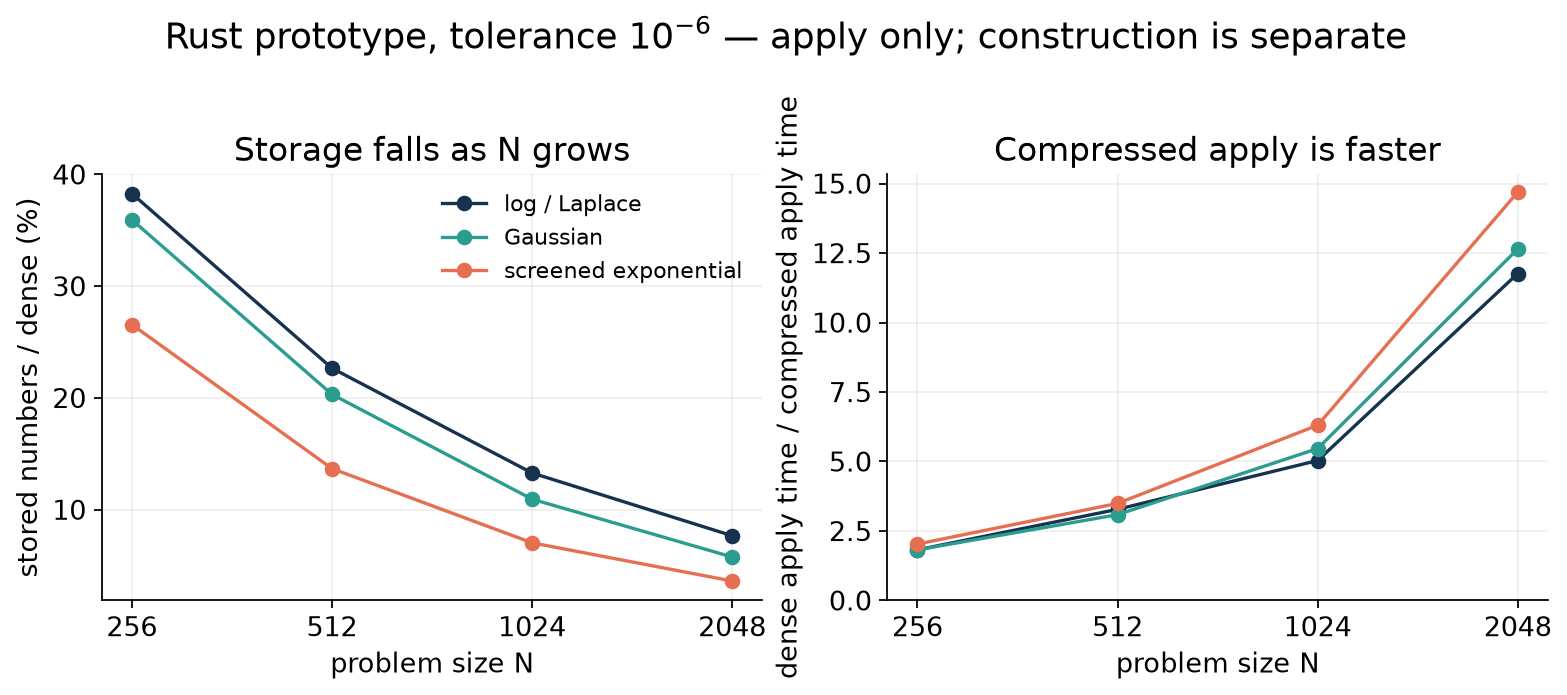
\includegraphics[width=\linewidth]{figures/rust-scaling.png}
\caption{Compressed storage decreases as a fraction of dense, while repeated apply becomes faster. Construction is reported separately.}
\label{fig:rustscaling}
\end{figure}

Compression itself took about $0.96$ seconds per problem at $N=2048$; dividing by the measured saving per call gives an estimated break-even after roughly 1,560, 1,619 and 1,559 applies for log/Laplace, Gaussian and screened exponential respectively. These are \textbf{dense-to-compressed oracle factors}, best suited to repeated apply: construction is not a fast hierarchical builder. Raw samples, min/median values and peak RSS are in \path{rust/results/summary.json}.

The exact DFT-butterfly example at $N=1024$ has $22{,}528=2N\log_2N+2N$ stored entries, every stage rank one and relative error $1.83\times10^{-16}$ against a separate FFT. The main Rust crate has 21 recorded passing checks. The broader core prototype has 72 exact golden values and 17 explicitly documented QR-tolerance-boundary count differences. Its recorded errors remain below $10^{-8}$ and LU residuals are at most $1.724\times10^{-15}$. Parity is judged by achieved accuracy rather than bit-identical rank counts.

For the Python generic B1 butterfly, stored entries/dense at $N=4096,t=1$ are $0.116$ at $\eps=10^{-6}$ and $0.150$ at $\eps=10^{-8}$. These ratios describe that driver and tolerance, not every oscillatory operator.

\subsection{Checked boundaries behind those measurements}
The boundaries are best stated as capabilities and evidence, not as an apology for what is absent:
\begin{itemize}
 \item \textbf{Python:} 126 recorded core tests pass, including all seven restored reference-SVD comparisons; 24 showcase tests pass; 10 spherical-harmonic tests pass after the corrected Gauss-node regression. The collection count of 264 is not an all-long-tests-pass claim.
 \item \textbf{Reference construction:} the Python recursive driver and main Rust dense-to-compressed path retain dense working matrices. They demonstrate achievable factors and solves but do not certify dense-free $O(N\log N)$ construction.
 \item \textbf{Rust coverage:} real scalar apply examples and the separate broader feasibility core are checked. One production-wide Rust API, deliberate production LAPACK selection, the complete physics experiments' special functions, and a matched-backend language-speed comparison are not established.
 \item \textbf{Method coverage:} FMM and wideband FMM are fully explained in the report through their expansion/translation roles; their production operators are not silently attributed to the small reference libraries.
\end{itemize}
Exact provenance and per-suite commands are recorded in these guides:
\begin{itemize}
 \item \path{python/docs/STATUS.md} and \path{python/docs/TESTING.md};
 \item \path{rust/PORT_STATUS.md} and the receipts under \path{results/}.
\end{itemize}

\section{Conclusion: one strategy, many algorithms}
The framework's most useful contribution is not a menu from which any solver follows automatically. It is a common way to \textbf{read, diagnose and test} a hierarchical method:
\begin{enumerate}
 \item Find an interaction matrix's useful groups and orderings.
 \item Decide which interactions a short representation can describe safely.
 \item Derive or choose that representation, with rank/error evidence.
 \item Obtain it through an honest sampling/access model.
 \item Assemble it by the relevant translation, sparse-factor recursion or elimination, and measure build, storage, apply and stability separately.
\end{enumerate}
FMM and wideband FMM make grouped summaries powerful through expansions and scale-specific translations; HBS/RS and FMM-LU turn them into direct solves through elimination and modified-block bookkeeping; butterflies use complementary tilings and nest local bases; the FFT combines exact residue-class rank one with Cooley--Tukey recursion.

The twelve experiments show the essential research motion: a generic choice works until an identifiable hypothesis fails, and the failure points to the new mathematics---not to a universal ``next solver''. Sometimes that mathematics is an adjoint identity, a richer proxy geometry or a two-sided coefficient. Sometimes it is a negative cost result telling us not to make the proposed change. The shared framework organizes the problem and the evidence; the application-specific mathematics still solves it.

\appendix
\section{One additional Matérn identity}
\label{app:matern}
For $f_\mu(r)=(\kappa r)^\mu K_\mu(\kappa r)$, where $K_\mu$ is the modified Bessel function of the second kind,
\begin{equation}
 (\kappa^2-\Delta_D)f_\mu(r)
 =\kappa^2(2\mu+D-2)f_{\mu-1}(r),\qquad r>0.
 \label{eq:matern-identity}
\end{equation}
The coefficient vanishes at $\mu=1-D/2$, explaining when the chain of related kernel orders terminates in a compatible dimension. With $\beta=\lceil\nu+1\rceil$ and $D=2(\beta-\nu)$, a finite integer-dimensional local lift in this construction requires $2\nu\in\mathbb Z$. Formal fractional dimensions are not a completed PDE proof.

For the unscaled convention $r^\mu K_\mu(\kappa r)$, the corresponding factor is $\kappa$, not $\kappa^2$. This is only a normalization difference in writing the same radial function.

\section{Experiment evidence by problem and source directory}
\label{app:experiments}
\begin{longtable}{@{}>{\raggedright\arraybackslash}p{0.20\textwidth}>{\raggedright\arraybackslash}p{0.40\textwidth}>{\raggedright\arraybackslash}p{0.30\textwidth}@{}}
\toprule
Experiment & Main control and reading & Evidence in \texttt{python/unified/explore/}\\
\midrule
\endhead
Interaction geometry & Compare admissibility geometry and storage at the same kernel. Do not treat nested butterfly storage as identical to an ordinary flat H-matrix convention without distinguishing formats. & \path{e1_which_structure/findings.md}; \path{results/storage_vs_N.png}. \\
DFT/FFT replacement & Natural versus bit-reversed DFT tiles. Both orderings matter, but generic tile rank alone doesn't furnish Cooley--Tukey recursion. & \path{e2_fft_replacements/findings.md}; \path{fig_a_nnz.png}. \\
Compressor swaps & Surface/volume proxy comparisons and non-PDE kernels. Use equal achieved errors and appropriate sample geometry. & \path{e3_compression_swaps/findings.md}; \path{e4_nonpde.png}. \\
Butterfly in a solver & Oscillatory butterfly application during the solve. Check the effect on iterative steps and distinguish it from a direct butterfly factor. & \path{e4_butterfly_in_solver/findings.md}; \path{gmres.png}. \\
Complex Helmholtz & Ordinary versus adjoint row step, with high-wavenumber pivot checks. Severity is regime-dependent; this isn't a universal indictment of FMM-LU. & \path{e5_highk_instability/findings.md}; \path{r1_ksweep.png}. \\
Stokes flow & Compare per-box, per-dof and total-storage statistics. Use zero-net-force or periodic benchmarks rather than the convention-dependent settling plot. & \path{e6_stokes/findings.md}; \path{r2_ranks.png}. \\
Screening and heat & Absolute versus relative tolerance under screening, and $\kappa\to0$ spectral control. Boundary-only heat representation has explicit source/initial-data scope. & \path{e7_yukawa_heat/findings.md}; \path{r3_quadrature.png}. \\
Fractional/Riesz interactions & Point count versus sample coverage. An annulus can work as well as a hemisphere. ``Two latitudes suffice'' in one solve is not a per-box $\eps$ theorem. & \path{e8_fractional/findings.md}; \path{r2_sweep.png}. \\
Lippmann--Schwinger scattering & Contrast evaluated on correct versus wrong sampling side. Smooth and piecewise-constant contrasts have different rank effects. & \path{e9_lippmann_schwinger/findings.md}; \path{r0_verify.png}. \\
Spherical harmonics & Turning-line rank, Gauss-transpose exactness, absolute-tolerance handling. Test the protective guard rather than depending on a platform-specific raw NaN. & \path{e10_sht_butterfly/findings.md}; \path{r4_turning_map.png}. \\
Matérn covariance & Circle refinement, kernel order and integer-$\nu$ controls. Track conditioning and posterior metrics, not just compression error. & \path{e11_matern/findings.md}; \path{r1_table.png}. \\
Oseen wakes & Stream-aligned versus cross-stream admissibility, depth-sensitive cost, and drag functional versus raw-density conditioning. & \path{e12_oseen/findings.md}; \path{r2_admissibility.png}. \\
\bottomrule
\end{longtable}
The independent audit \path{results/update-review.md} records exact controls and corrections. Directory prefixes below are retained only as evidence identifiers, not as experiment titles.

\clearpage
\section{Reproduction guide}
\label{app:reproduce}
Run from \path{deliverables/}. Both implementations are independent of the original supplied \path{source/} and \path{updated/} archives. No cache or generated build directory is needed.

\subsection*{Python}
Requires Python 3.12+, NumPy, SciPy, Matplotlib; pytest for tests.
\begin{lstlisting}[language=bash]
cd python
python3 -m pip install -e '.[test]'                   # optional setup
scripts/collect-tests.sh
scripts/test-core.sh
scripts/test-showcase.sh
scripts/test-all.sh                                  # all twelve research suites; longer
PYTHONPATH=. python3 -m unified.showcase.reproduce --quick --no-write
scripts/build-wheel.sh
\end{lstlisting}
The wrapper scripts set the correct package import path and pin the main BLAS variables to one thread. The optional comparison baseline is now packaged as \path{unified.reference.butterfly}, so it does not depend on an absent original \path{code/} directory. The shared \path{core/*.py} files are unchanged; distribution edits are the reference-loading path, the corrected spherical-harmonic Gauss-node sign and the backend-independent spherical-harmonic test. See \path{docs/PROVENANCE.md}.

Saved figures and result tables are in \path{unified/explore/*/results/}. Inspecting them requires no long regeneration. Full-suite timing depends on the machine and solver settings; \path{264} is a test collection count, not a claim that every long research test completed.

\subsection*{Rust}
Built and tested with Rust 1.93.1.
\begin{lstlisting}[language=bash]
cd rust
cargo test --release --workspace --all-targets
cargo run --release --example laplace -- 2048
cargo run --release --example dft_as_butterfly
scripts/run.sh
\end{lstlisting}
\path{run.sh} stores kernel sweeps, direct FFT comparisons, exact DFT output and the reference-core golden logs under \path{results/}. The broader core's 17 tolerance-boundary count differences are intentional findings with separately checked achieved errors, not a hidden build failure.

\subsection*{Report and slides}
\begin{lstlisting}[language=bash]
python3 scripts/make_figures.py
cd latex
latexmk -pdf -interaction=nonstopmode -halt-on-error report.tex
latexmk -pdf -interaction=nonstopmode -halt-on-error slides.tex
\end{lstlisting}
\path{main.pdf} is a compiled copy of this report. \path{slides.pdf} contains the eight-minute deck, and \path{latex/speaker-notes.md} supplies a roughly seven-minute spoken script with pause transitions. All report figures can be rebuilt from the included data by \path{scripts/make_figures.py}.

\begin{thebibliography}{99}\small
\bibitem{li2015butterfly} Y. Li, H. Yang, E. R. Martin, K. L. Ho, L. Ying.
\emph{Butterfly Factorization}. Multiscale Modeling \& Simulation \textbf{13}(2), 2015.
\url{https://arxiv.org/abs/1502.01379}.
Reference for the middle-level split, nested bases, randomized constructors and complexity.

\bibitem{candes2009butterfly} E. Candès, L. Demanet, L. Ying.
\emph{A Fast Butterfly Algorithm for the Computation of Fourier Integral Operators}. SIAM Multiscale Modeling \& Simulation \textbf{7}(4), 2009.
\url{https://arxiv.org/abs/0809.0719}. General complementary low-rank analysis and its phase-regularity hypotheses.

\bibitem{cheng2006wideband} H. Cheng et al.
\emph{A wideband fast multipole method for the Helmholtz equation in three dimensions}. Journal of Computational Physics \textbf{216}(1), 2006.
\url{https://amath.colorado.edu/faculty/martinss/2014_CBMS/Refs/2006_rokhlin_wideband.pdf}.
Source for multiple stable expansion families, diagonal translation, conversion and the scale-dependent switch.

\bibitem{ho2012hife} K. L. Ho, L. Greengard.
\emph{A fast direct solver for structured linear systems by recursive skeletonization}. SIAM Journal on Scientific Computing \textbf{34}(5), 2012.
\url{https://arxiv.org/abs/1110.3105}. Weak-interaction recursive skeletonization.

\bibitem{minden2017rss} V. Minden, K. L. Ho, A. Damle, L. Ying.
\emph{A recursive skeletonization factorization based on strong admissibility}. Multiscale Modeling \& Simulation \textbf{15}(2), 2017.
\url{https://arxiv.org/abs/1609.08130}. Strong interaction and modified-block bookkeeping.

\bibitem{sushnikova2023fmmlu} D. Sushnikova, L. Greengard, M. O'Neil, M. Rachh.
\emph{FMM-LU: A fast direct solver for multiscale boundary integral equations in three dimensions}. Journal of Computational Physics \textbf{476}, 2023.
\url{https://arxiv.org/abs/2201.07325}. Tree organization, modified blocks, quadrature and proxy analysis for a complete 3-D boundary solver.

\bibitem{pang2018idbf} Y. Pang, K. L. Ho, H. Yang.
\emph{Interpolative Decomposition Butterfly Factorization}. SIAM Journal on Scientific Computing \textbf{42}(2), 2020.
\url{https://arxiv.org/abs/1809.10573}. Column-selecting bases and sampled-row construction routes.

\bibitem{cooley1965fft} J. W. Cooley, J. W. Tukey.
\emph{An algorithm for the machine calculation of complex Fourier series}. Mathematics of Computation \textbf{19}(90), 1965.
\url{https://doi.org/10.1090/S0025-5718-1965-0178586-1}. Classical radix-2 Cooley--Tukey factorization.

\bibitem{oneill2010butterfly} M. O'Neil, F. Woolfe, V. Rokhlin.
\emph{An algorithm for the rapid evaluation of special function transforms}. Applied and Computational Harmonic Analysis \textbf{28}(2), 2010.
Interpolative butterfly construction with skeleton columns and equivalent weights.

\bibitem{projectaudit} This project.
\emph{Independent framework audit and post-update experiment review}.
Included with this submission in \path{results/}: \path{framework-explained.md} and \path{update-review.md}, plus rerunnable checks in \path{results/verification/}.
\end{thebibliography}
\end{document}
